In this sector, we modified the settings for the maximum running map/reduce tasks in one slave machine, which is called "map/reduce slot number". We set both the value for map and reduce to 8, and makes the threshold for 300MB. As in our test cluster, each slave machine has only 2GB physical memory, the experiment shows the result how hadoop acts in this case. Note that we also modified the JVM Xmx value to 700MB which avoids the memory failure caused by JVM that has been tested in section 4.2.3. We also use the four types of memory behavior as the test applications. 

\begin{figure}[ht]
  \centering
    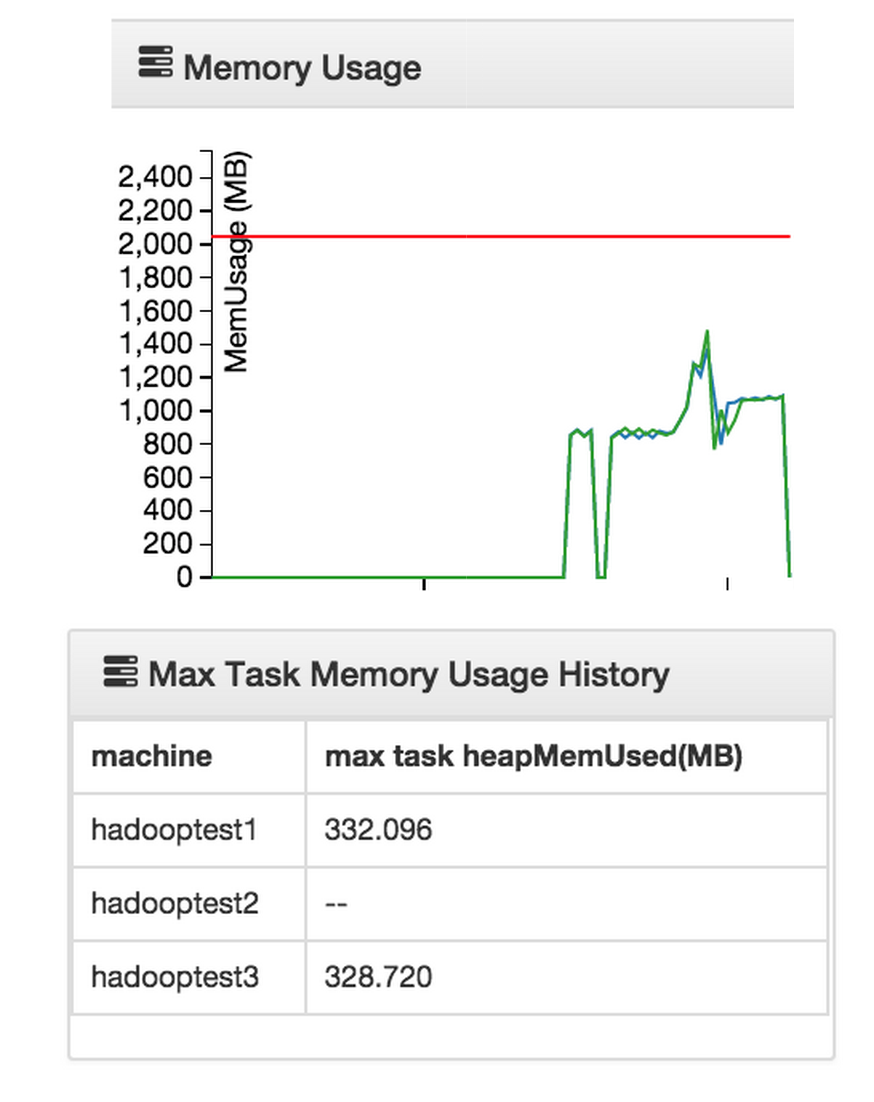
\includegraphics[width=2.1in]{image/test3a.png}
    \caption{Memory Usage under Same Threshold without Clearance}
    \label{ref:test3a}
\end{figure}

In Figure 17, the tested memory behavios is "Same Threshold without Clearance". The whole job failed with error message "there is insufficient memory for the Java Runtime Environment to continue. Native memory allocation (malloc) failed to allocate committing reserved memory." This error makes Child JVM exits with error, as it cannot get enough memory. As we set each mapper's threshold 300MB, and there are 8 mappers running at the same time which will need more than 2GB memory, but the physical space is just 2GB, so in this case all of the mappers will fail as they all cannot get enough memory to continue.

\begin{figure}[ht]
  \centering
    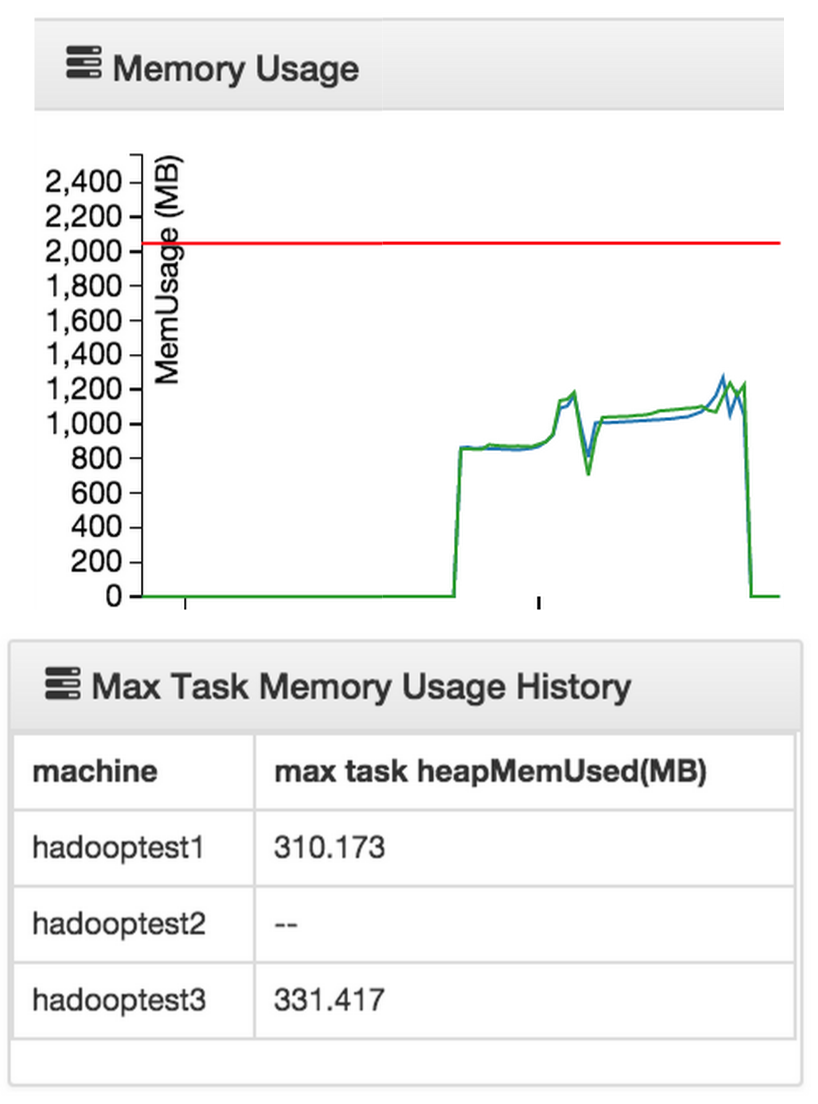
\includegraphics[width=2.1in]{image/test3b.png}
    \caption{Memory Usage under Random Threshold without Clearance}
    \label{ref:test3b}
\end{figure}

In Figure 18, the tested memory behavior is "Random Threshold without Clearance". Even though the threshold is randomized and smaller than 300MB, but some of the mappers still cannot get enough memory for their own threshold, which will cause the child error, and the retry might success, but also might fail. Too many tasks failure will cause the whole job fail, and then it stops.

\begin{figure}[ht]
  \centering
    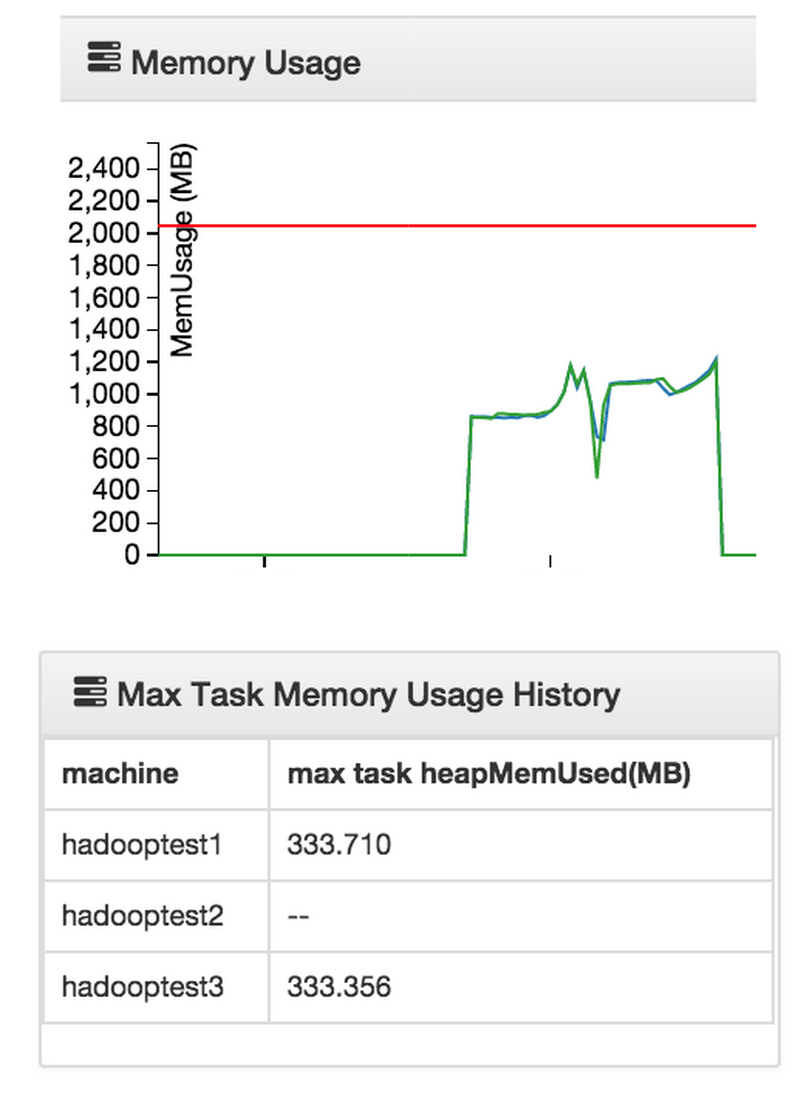
\includegraphics[width=2.1in]{image/test3c.png}
    \caption{Memory Usage under Same Threshold with Clearance}
    \label{ref:test3c}
\end{figure}

In Figure 19, the tested memory behavior is "Same Threshold with Clearance". It still cannot run successfully. As the setting for the threshold is 300MB, none of the maptask can read 300MB and starts to clear the data they hold. Here in this case, it is almost the same with shown in both Figure 17 and Figure 18. As all the mappers are trying to get more data as they can, but the more they want, the easier they fail.

\begin{figure}[h]
  \centering
    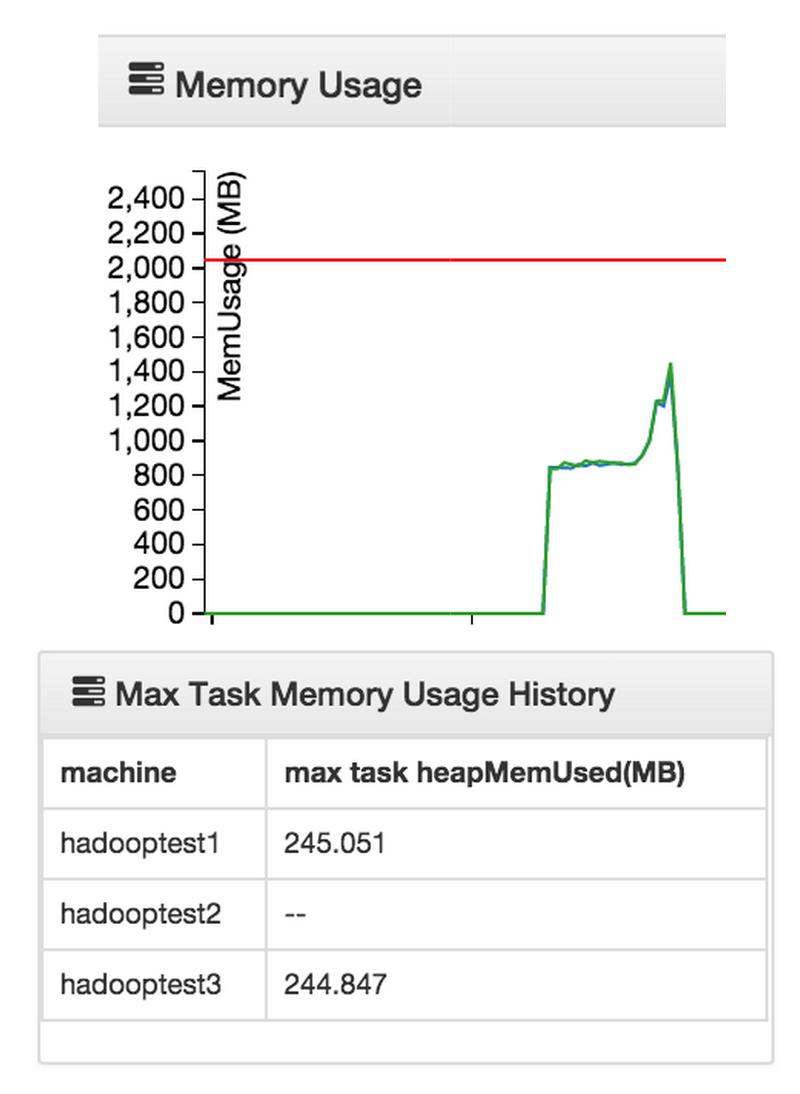
\includegraphics[width=2.1in]{image/test3d.png}
    \caption{Memory Usage under Random Threshold with Clearance}
    \label{ref:test3d}
\end{figure}

In Figure 20, the tested memory behavior is "Random Threshold with Clearance". It still show failure the same with the former three ones. 